\documentclass[../main]{subfiles}
\bibliography{reference, reference_web}
\graphicspath{{../figures/}}

\begin{document}


% 図表の例:コーンペネトロメータを\reffig{fig:cone_penetrometer}に示す.
% \reftab{tab:traffic_cone_index}が示すように,各建設機械の走行に必要とされているコーン指数は既にわかっている.

\section{背景}
\label{sec:intro_background}
\subsection{石油精製プラント点検の現状}
\label{sec:intro_plant_current}


近年,地球温暖化の進行を抑えるため,カーボンニュートラルの実現が求められている.
しかし,\reffig{fig:oil_consumption}に示されるように,石油をはじめとする化石燃料は,将来的にもエネルギー源として重要な役割を果たすと予想されている\cite{ritchie2023energy}.

石油の精製は,ガソリン,ディーゼル燃料,ジェット燃料などの輸送用エネルギー資源だけでなく,プラスチック,化学肥料,医薬品,合成繊維など,幅広い化学製品を生み出すために欠かせない工程である.その中心的役割を担うのが,\reffig{fig:view_plant}に示す石油精製プラントであり,施設内にはポンプ,熱交換器,蒸留装置,配管など多種多様な装置が複雑に組み合わさって存在している.\cite{eneos2024,Shvindin2008A}
これらの装置が適切に稼働することで,高品質なプロダクトが安定して供給され,産業や社会の基盤を支えている.

一方,保守作業はどの産業においても重要な要素であり,石油精製プラントも例外ではない.
設備は老朽化や環境条件による劣化で故障することがあり,その結果,操業停止による生産遅延,修理費の増加などの損失が発生する.
さらに,石油精製プラントでは可燃性物質を多数扱うため,他の産業施設に比べて火災や爆発など重大な事故が発生するリスクが高く,その被害は甚大になり得る\cite{Tang2021105623}.
こうしたリスクを低減するためには,設備の異常を早期に発見し,適切な対策を講じることが求められる.

現状では,石油精製プラント内の設備点検は専属の現場作業員が定期的な巡回で行い,視覚・聴覚・嗅覚・触覚による異常の有無の確認が基本である.
こうした点検は1日に4~5回実施され,昼夜を問わず行われているため,夜間作業による負担や,高齢化による熟練人材の不足,熟練度の差による点検品質のばらつきといった様々な課題が生じている.
これらの理由から,プラント内点検の自動化が求められている.

\subsection{固定センサを用いた点検と移動ロボットを用いた点検}

プラント内点検の自動化には,大まかに以下の2つのアプローチが存在する.
1つは,固定センサを用いた点検であり,もう1つは,移動ロボットを用いた点検である.

固定センサを用いた点検の例として,Lv らの研究が挙げられる\cite{Lv2023Overview}.
Lv らはマイクをセンサとして用いてギアやポンプなどの機器から発する異常音を検知する手法を提案している.
固定センサを用いたアプローチには常時監視が可能というメリットがある一方で,いくつかの課題が存在する.
まず,石油精製プラント内では可燃性物質を多数扱うため,センサと解析に用いる装置をつなぐ通信線も含め,防爆仕様とする必要がある.
その結果,各センサの導入コストが高くなる.
さらに,広大なプラント全体を点検するためには多数のセンサを設置しなければならず,設置や維持にかかるコストも高くなる.


そこで近年では,移動ロボットを用いた点検が注目されている.
この手法では,点検に必要なマイクやカメラなどのセンサをロボットに搭載し,ロボットがプラント内を移動しながら,センサから情報を取得することで異常を検知する.
移動ロボットを用いた点検では,必要となるセンサの数がロボット台数に比例するため,固定センサを用いた点検と比べて,センサの設置コストや維持コストを低く抑えやすい.
また,石油精製プラントにおける現場作業員の点検を移動ロボットによる点検で代替することを目的とした移動ロボットの開発が盛んに行われている\cite{Shukutani2018}.

以上を踏まえ,本研究では移動ロボットを用いた点検に着目する.

\begin{figure}[t]
  \centering
  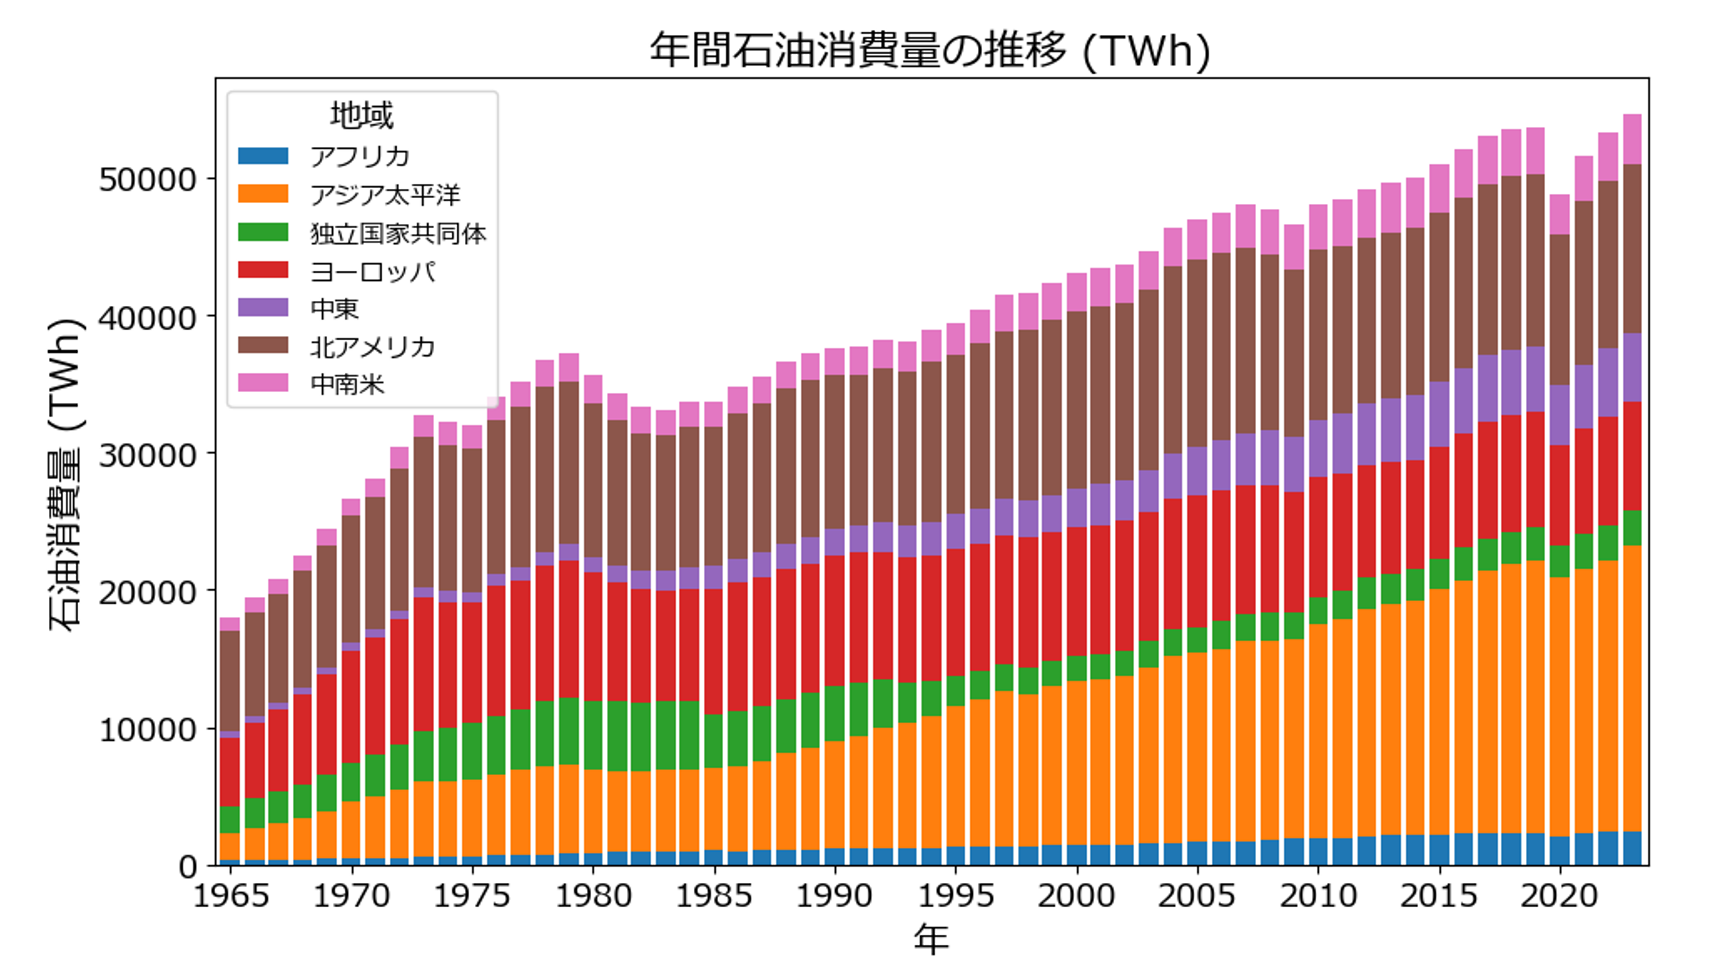
\includegraphics[keepaspectratio, width=1.0\linewidth]{chap1/oil_consumption.png}
  \caption{世界石油消費量の推移}
  \label{fig:oil_consumption}
\end{figure}

\begin{figure}[t]
  \centering
  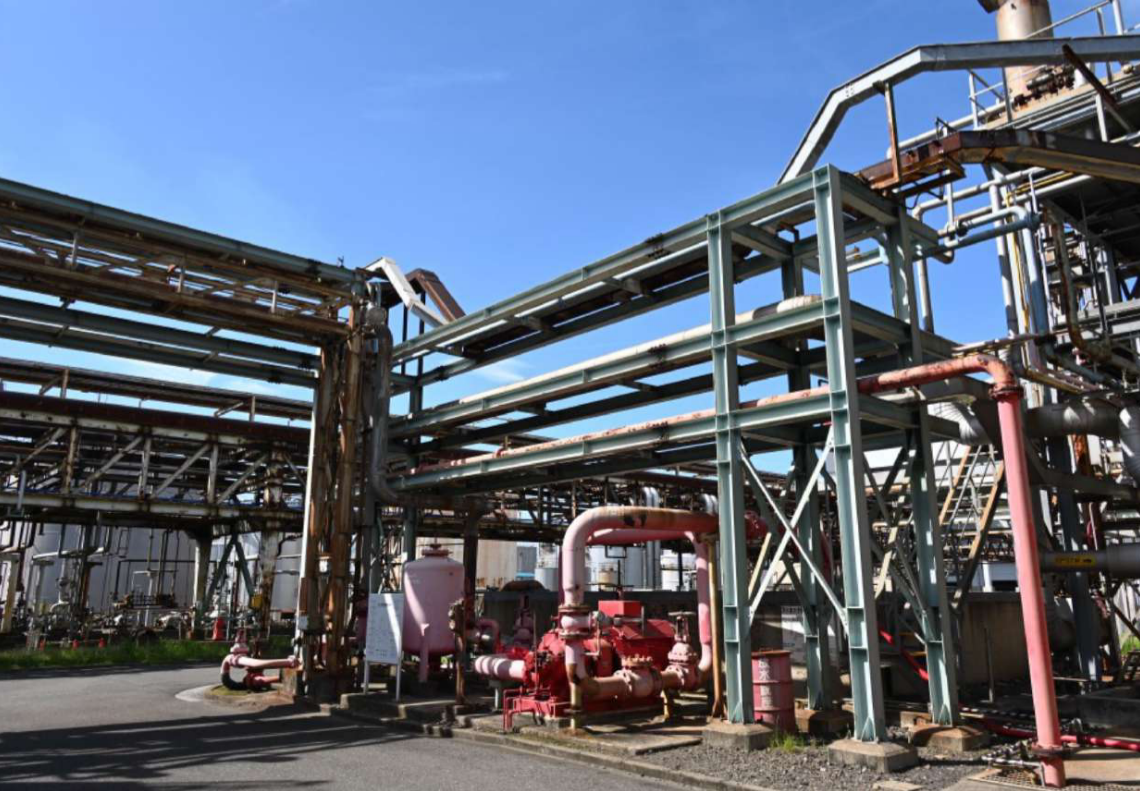
\includegraphics[keepaspectratio, width=0.8\linewidth]{chap1/view_plant.png}
  \caption{石油精製プラント}
  \label{fig:view_plant}
\end{figure}


\begin{table}[t]
  \caption{プラント内の異常の種類(株式会社ENEOSより提供)}
  \label{tab:plant_anomalies}
  \centering
  \begin{tabular}{lll}
    \toprule
    対象機器 & 監視対象 & 検査手法 \\
    \midrule
    ポンプの異常 & ベアリング異音 & 聴覚 \\
                 & 漏洩による白煙発生 & 視覚,嗅覚 \\
                 & 漏洩による着火 & 視覚,嗅覚 \\
                 & オイラーのオイルレベル低下 & 視覚 \\
                 & 閉塞等による冷却水低下、喪失 & 触覚 \\
                 & 発熱 & 触覚 \\
    \midrule
    配管異常 & 外面腐食の進行 & 視覚 \\
               & 保温板金の劣化 & 視覚 \\
               & 保温劣化による表面温度上昇 & 触覚 \\
               & 腐食によるガス・油漏洩 & 視覚,嗅覚 \\
               & フランジ部からのガス・油漏洩 & 視覚,嗅覚 \\
    \midrule
    その他機器の異常 & 加熱炉の耐火煉瓦脱落による炉壁発熱 & 視覚 \\
                   & バルブの誤開閉 & 視覚 \\
    \midrule
    メータ読み込み & 圧力計、温度計等 & 視覚 \\
    \bottomrule
  \end{tabular}
\end{table}



\subsection{ポンプを対象とした点検}
\label{sec:intro_plant_characteristics}


石油精製プラント内では,多様な装置が複雑に組み合わさり,経年劣化などを原因とした様々な異常が発生し得る.
\reftab{tab:plant_anomalies}に示すように,プラント内ではポンプや配管,その他の設備に関連した多種多様な異常が確認され,
それぞれの異常毎に適切な人間の感覚を用いた点検が行われている.


中でも,\reffig{fig:pump}に示すようなポンプはプラント内での液体やスラリー(液体と固体の混合物)の移動に用いられる装置であり,プラント内にて最も多く設置されている機器の1つである.
これらのポンプは内部に回転機構を有しており,その中核には流体を昇圧・輸送するための回転軸が配置されている.
回転軸の安定した回転を支えるため,ポンプ内部にはベアリングと呼ばれる部品が組み込まれている.
ベアリングは回転軸に掛かるラジアル(軸方向)およびスラスト(軸垂直方向)方向の加重を受け止め,摩擦を低減する役割を担う.

しかし,ポンプが長時間稼働を続ける中で,主にベアリング内部のグリースの不足が原因となり,
ベアリングは次第に摩耗し,その性能を劣化させていく.
ベアリングの摩耗が進行すると,騒音や異常な温度上昇が起こるだけでなく,軸の振れ周りの振動が大きくなり,
ポンプ全体の異常停止や,ポンプの破損につながる可能性がある.
特に石油精製プラントのような安定操業が求められる現場では,ポンプ内のベアリング摩耗は極力未然に防止検知することが重要である.

現在石油精製所内での巡回点検では,ポンプの異常を検知するために聴覚を用いた点検が行われている.
現場作業員は,\reffig{fig:monitoring}に示すように,点検の対象となるポンプに近づくことで,
それらの機器から発生する音を基に異常の有無を検知している.
ベアリング内部のグリースが不足すると潤滑が十分に行われなくなり,金属同士が直接こすれあうことで摩擦音や金属音などの異音が発生し,
これを聴覚で検知することができる.

一方,振動計を用いた異常検知手法も研究されている\cite{SMITH2015100}.
Smithらは,振動計で計測した振動パターンを解析することで,ベアリングの摩耗や異常を検知する手法を提案している.
ただし,この手法は直接接触による情報取得が前提となるため,コンタクトレスな点検が不可能であり,移動ロボットとの適合には課題がある.



さらに,近年では清水らによる研究において,移動ロボットに搭載したカメラを用いてプラント機器の監視と異常検知を行う手法が提案されている\cite{shimizu2024change}.
しかし,ポンプ内部のベアリングは筐体内部に設置されているため,視覚情報の取得が遮蔽(オクルージョン)の問題で困難となる.
そのためカメラベースの手法をそのままポンプ内部のベアリングを対象とした異常検知に適用することは難しい.

以上を踏まえ,\reftab{tab:synthesis}に,移動ロボットの適合性や筐体内部情報の取得可能性の観点から,振動計,カメラ,マイクロホンを用いた点検手法を比較した結果を示す.

本研究では,空気を媒体とする音響信号は遠方からでも取得可能であるため移動ロボットとの適合性が高く,筐体内部の摩擦音や金属音といった情報も得やすいことに着目し,
マイクロホンによって取得される音響信号を用いた点検手法に焦点を当てる.



\begin{table}[htbp]
  \centering
  \caption{点検手法の比較}
  \label{tab:synthesis}
  \begin{tabular}{cccc}
  \toprule
  点検手法           & 筐体内部の点検& コンタクトレスな点検 \\ \hline
  振動計              & 〇                     & ×                   \\
  カメラ             & ×                     & 〇                   \\
  マイクロホン     & 〇                     & 〇                  \\ \bottomrule
  \end{tabular}
\end{table}

\begin{figure}[t]
  \centering
  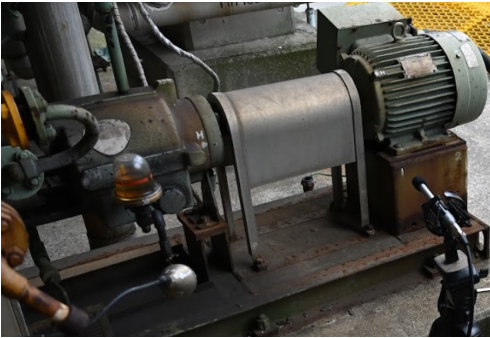
\includegraphics[keepaspectratio, width=0.8\linewidth]{chap1/pump.pdf}
  \caption{石油精製プラント内におけるポンプ}
  \label{fig:pump}
\end{figure}

\begin{figure}[t]
  \centering
  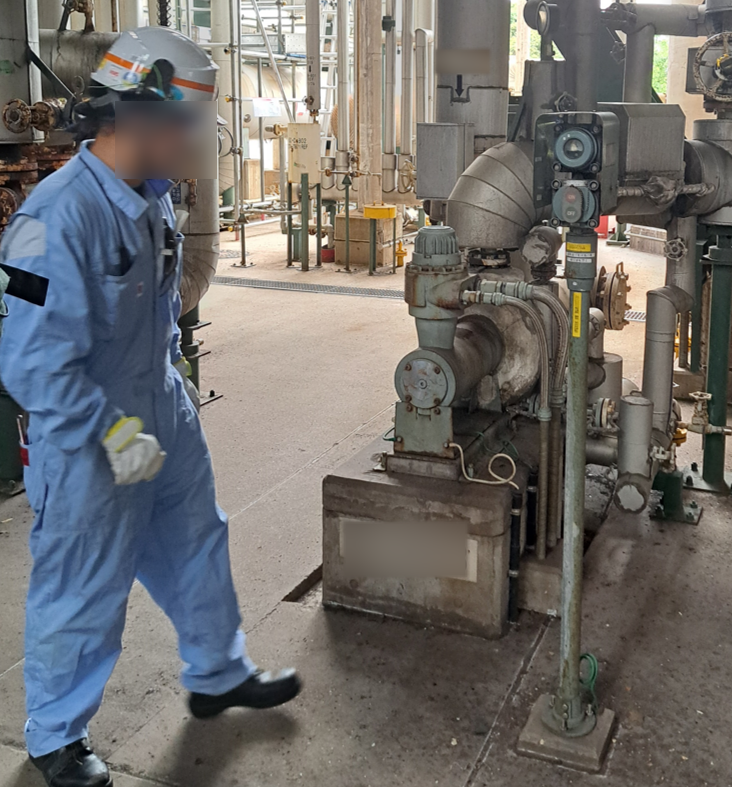
\includegraphics[keepaspectratio, width=0.8\linewidth]{chap1/monitoring.png}
  \caption{現場作業員による聴覚を用いたポンプの点検の様子}
  \label{fig:monitoring}
\end{figure}
\end{document}
